\section{Binary ion solutions}
Batch filtrations of solutions of either \ce{NaCl}, \ce{CaCl2} or \ce{Na2OSiO2} was performed according desrcibtion presented in \rod{XX}. 
%The solutions were prepared by adding each salt to the required amount of RO water.
%Due to the nature of the filtration setup the feed tank was left open to the air during the filtration process.
The ionic rejections were (more or less) stable during the 4.5 hours of filtration and is calculated as an average of the filtration.
The rejections of anions, cations and \ce{SiO2} are compared in \cref{fig:single_salt_avg_rejecion_comparison_bar} and from these results it is evident that the salt has an influence on the rejection of the various ions. 
The chloride rejection is influenced by the corresponding cations present; when monovalent sodium ions are present the average rejection is  15.9 \%, which is increased to 56.7 \% when the anion is switched to calcium which is divalent.

\begin{figure}[htbp]
    \centering
    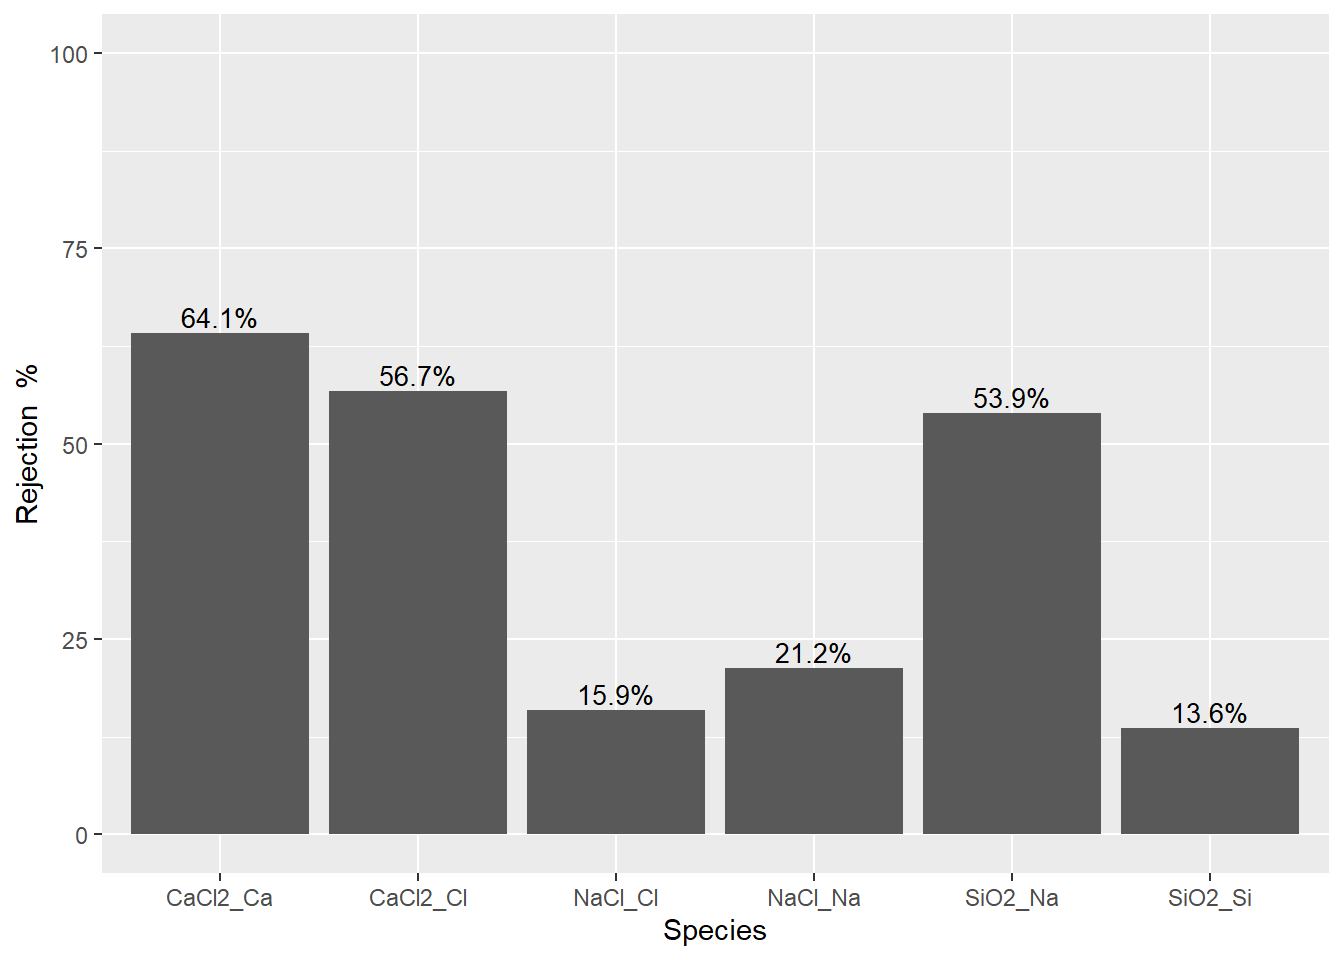
\includegraphics[width=0.7\textwidth]{Billeder/data/single_salt/rejection_singlesalt_barplot.png}
    \caption{Rejection of anions, cations and \ce{SiO2}, }
    \label{fig:single_salt_avg_rejecion_comparison_bar}
\end{figure}

\textcolor{blue}{Sebastians rapport} ran filtration of similar compositions using a similar membrane in a single pass setup.
The results obtained are presented in \Cref{tab:single_salt_rejection_sebastian_comparison} along with the result obtained in this work.
From this it is evident that this batch filtration achieved a lower rejection of ions than the single pass filtrations.

\begin{table}[h]
\centering
\caption{Rejection of ions from filtration of binary ionic mixtures}
\begin{tabular}{c|cc|cc|cc|cc|cc}
Salt & \multicolumn{2}{c|}{\ce{NaCl}} & \multicolumn{2}{c|}{\ce{CaCl_2}} & \multicolumn{2}{c}{\ce{Na_2SO_4}} & \multicolumn{2}{c|}{\ce{CaSO_4}} & \multicolumn{2}{c}{\ce{Na_2SiO_3}} \\
Ion & \ce{Na+} & \ce{Cl-} & \ce{Ca^{2+}} & \ce{Cl-} & \ce{Na+} & \ce{SO_4^{2-}} & \ce{Ca^{2+}} & \ce{SO_4^{2-}} & \ce{Na+} & Silica \\ \hline
our rejections [\%] & 15.9 & 21.2 & 64.1 & 56.7 & - & - & - & - & 53.9 & 13.6 \\
seb's rejections [\%] & 35 & 37 & 69 & 68 & 98 & 99 & 97 & 98 & - & -   \label{tab:single_salt_rejection_sebastian_comparison}
\end{tabular}
\end{table}



\textbf{Charge discrepancy}
It is also evident that there is a discrepancy in rejections of each ion from a salt.
\textcolor{blue}{Sebastians rapport} saw similar rejection for the cation and anions from the same salt.
Due to the assumed charge balance over the membrane the expected result is to find similar retention of anions and cations, especially in the simplified case of one dissolved salt.
For the case of NaCl \textcolor{blue}{Sebastians rapport} found chloride and soidum rejections of 37 and 35 percent respectively. 
Ignoring the difference in performance seen by our results the large difference in charge balance: 16 percent rejection of sodium and 21 percent rejection of chloride is still at odds with the results.
\textcolor{blue}{Sebastians rapport} ran a single pass configuration at greater permeate flux (30 LMH) which could explain some of the performance differences, but still not the apparent charge non-neutrality.\\

\textbf{Concentration discrepancy}
\textcolor{magenta}{De værdier der er blevet målt stemmer ikke overens med det der er kommet i, skal det med i rapporten? who knows?}



\textbf{pH discrepancy}
\textcolor{magenta}{pH go down bad, we use buffer now!}
Before every experiment pH of the feed solution was adjusted with 2M \ce{HCl} or 2M \ce{NaOH} to the desired pH of 8.5.
During the filtration pH was logged and the results are shown in \Cref{fig:single_salt_pH}.
The measured pH varies between each solution, even after initial adjustment to pH 8.5, only the silica solution was still at pH 8.5 when the filtration started.
This indicates that the silica solution is more a more buffered solution than the other solutions. 
For the two salt solutions \ce{NaCl} and \ce{CaCl_2} pH decreased as the filtration progressed while it remained constant for the silica solution, which is another indicator that the buffering capacities differ between the solutions.

\begin{figure}[htbp]
    \centering
    \includegraphics[width=0.7\textwidth]{Billeder/data/single_salt/singlesalt_pH.png}
    \caption{pH during filtration }
    \label{fig:single_salt_pH}
\end{figure}

\textbf{Bicarbonate discrepancy}
\textcolor{magenta}{når man kommer silica i vand er der pludeslig mere bicarbonat i, det var da mystisk}
Along with measuring the concentrations of the ions which constitute the added salts the bicarbonate content of the feed tank was also analysed. 
Progression of measured bicarbonate content is shown in \cref{fig:single_salt_bicarbonate} for each of the experiments.
For each experiment bicarbonate concentration increases in the feed container as the experiment progressed \rod{specific values}.
There is a large difference in the initial bicarbonate concentration between the solutions of dissolved salts and the experiment on the silica solution.
The analysis of bicarbonate is based on a titration to specific pH where bicarbonate content is assumed to be directly proportional to the volume of acid required to reach the target pH.
As the solutions of silica likely are more buffered than the other solutions the analysis may be a result of the greater buffer capacity of the solution rather than an increased bicarbonate content.  




\begin{figure}[htbp]
    \centering
    \includegraphics[width=0.7\textwidth]{Billeder/data/single_salt/singlesalt_bicarbonat.png}
    \caption{Analysed Bicarbonate content}
    \label{fig:single_salt_bicarbonate}
\end{figure}





\textcolor{magenta}{Old stuff (maybe incorporate):}

The TMP was calculated from the experiment with NaCl where the initial TMP is \rod{2.5 bar} which decrease slightly over the duration of the experiment to \rod{about 2.3 bar}. \textcolor{blue}{why decrease}
increase in flucturations this was due to a mistake during there experiment were air was introduced to the system, as the feed tube was exposed to air. This reduced the effect of the pressure dampeners as they were filled with air instead of water. 
\textcolor{blue}{noget med højere rejection måske det skyldes de der divalente ioner.}






% \begin{table}[H]
% \centering
% \caption{Stats fra single salt experiment }
% 	\begin{tabular}{c|cc}
%     Species & Concentration [mM]  & TMP [bar] \\ \midrule
%      \ce{NaCl} & 3  & 2.5-2.2\\
%      \ce{CaCl2}  &\rod{3} & 2.5 \\
%      \ce{Na2SO4}  &  1 &\\
%      \ce{CaSO4} &  1&\\
%      \ce{Na2OSiO2}  & 1 & \\
%      	\end{tabular}
% 	\label{Tab:single_salt_conc_pressure}
% \end{table}